\chapter{Installing Hobbit}
\section{Installing Hobbit}


 This describes how to setup a Hobbit server for monitoring your
 systems. It assumes that you are setting up a full Hobbit server -
 i.e. either you do not have a Big Brother server, or you will replace
 it completely with Hobbit.



 Note to Big Brother users: Although some of the Hobbit tools have evolved from the bbgen toolkit that was used on top of a Big Brother server installation, the Hobbit versions of these tools now require that you run Hobbit - not Big Brother. If you are migrating from Big Brother to Hobbit, then you should follow the migration guide.
\subsection{Prerequisites - before you install Hobbit}


 There are a few things you should check before you begin to install Hobbit. Dont be scared of the number of items here - it is likely that you already have most or all of it in place.
\textbf{A webbrowser capable of handling HTML 4, JavaScript and CSS}


 This includes most browsers available today - Internet Explorer 5 or later, all Mozilla/Firefox versions, Konqueror, Netscape 6 and several others. The old Netscape 4.x browsers are known NOT to work.
\textbf{A Unix-like operating system}


 Hobbit is written for Unix-based systems, e.g. Linux, FreeBSD, or Solaris. It will probably work on any Unix-like system that supports the Unix System V IPC mechanisms (shared memory, semaphores) - that should be just about anything Unix-like you are likely to have.
\textbf{Sufficient SYSV IPC ressources on your system}


 Hobbit uses 8 shared memory segments, ranging in size from 32 KB to 512 KB (2336 KB total) in the default configuration; and 8 sets of 3 semaphores. Experience shows that some systems need tuning to provide the necessary IPC ressources that Hobbit uses. Specifically, when installing on Solaris you must increase the ``shmseg'' kernel parameter from the default 6 to at least 8. Since other programs on your system may also use shared memory, a higher value may be required. See \url{http://www.hswn.dk/hobbiton/2005/08/msg00183.html} for more information about these issues.
\textbf{A webserver}


 Hobbit is designed with a web-based front-end. So you should have a webserver such as Apache running on the server where you install Hobbit.
\textbf{A working C compiler, GNU make.}


 Hobbit is written in C, so you need a working C compiler, e.g. gcc. You will also need a ``make'' utility - many systems have one by default, but you need to use the GNU make utility. On some systems, this is pre-installed as ``gmake'' or ``gnumake''. The configure-script checks this for you.


 \textbf{HP-UX users}
 should note that the HP-supplied C compiler is known to mis-compile the lib/environ.c file, and produces an output file lib/environ.o of length 0 bytes. HP-UX users on the hobbit mailing list agree that the default C compiler shipped with HP-UX should not be used to compile Hobbit - it is only for re-building the HP-UX kernel. The GNU C compiler works fine on HP-UX. More details in this e-mail from the Hobbit mailing list.
\textbf{PCRE, RRDtool, libpng, OpenSSL, OpenLDAP, Net-SNMP libraries.}


 Hobbit relies on a number of Open-Source libraries - these must be installed before you start building Hobbit. On many systems you already have these pre-installed - they are commonly installed by default on Linux systems, and FreeBSD has all of them in the ``ports'' collection.


 Note: Although many systems have these libraries pre-installed, they often include only the run-time libraries and not the files that are needed to compile and build programs such as Hobbit. So if you think you have all of these libraries installed but Hobbit will not build, do check that you have the development files installed as well. Often these are in packages called ``something\emph{-dev}
``.
\begin{itemize}
\item PCRE - Perl Compatible Regular Expression library - is a library for matching text-strings. It is available from \url{http://www.pcre.org/}
\item RRDtool is a library for handling the Round-Robin Databases used to hold the historical data Hobbit gathers. It is available from \url{http://oss.oetiker.ch/rrdtool/}. Hobbit is known to work with RRDtool 1.0.x - if you prefer to use the newer RRDtool 1.2.x, make sure you use at least version 1.2.2.
\item libpng is a library for generating images in the PNG format. It is used by RRDtool (and hence Hobbit). You can find it at \url{http://www.libpng.org/pub/png/libpng.html}
\item OpenSSL is a library for communicating with network services, that use SSL encryption - e.g. secure websites. Although this library is not absolutely required for Hobbit, I strongly recommend that you install it because sooner or later you will probably need it anyway. It is available from \url{http://www.openssl.org/}. Note: If you are building on Solaris, you should check that you have a random-data generator, either the prngd daemon (available on Sun Freeware) or the Solaris /dev/random driver from Solaris patch 112438.
\item OpenLDAP is used to query LDAP directory servers. If you would like to test that your directory server is up and running, you will need this library. It is available from \url{http://www.openldap.org/}
\item Net-SNMP is used to query SNMP-based systems, typically network devices like routers, switches or firewalls. But nearly all types of computer systems have some sort of SNMP support. If you would like to collect data from SNMP-enabled systems you will need this library. It is available from \url{http://net-snmp.sourceforge.net/}

\end{itemize}


 The configure-script will attempt to locate all of these libraries on your system, and complain if the required ones are missing.
\textbf{A ``hobbit'' userid on your system}


 A core element of Hobbit is a network daemon. To keep your system secure and limit the amount of damage that can be done if someone finds a security problem in Hobbit, I strongly recommend that you create a dedicated userid for the Hobbit programs. This user should \emph{not}
 be a member of any other groups on your system.


 Hobbit will install the hobbitping tool as \textbf{setuid-root}
(only on the Hobbit server). This program requires root privileges to be able to perform network ``ping'' tests. It will drop root privileges immediately after obtaining the network socket needed for this, and will not run with root privileges at all while handling network traffic or doing file I/O. 
\subsection{Building Hobbit}


 After unpacking Hobbit from the tar-file, run the configure script. This script asks a series of questions, but all of the questions have a reasonable default response. So if you are in doubt about what to answer, use the default setting. You can see what it looks like.


 When the configure script finishes, it tells you to run make to build the Hobbit programs. If your default ``make'' tool is not GNU make, you should use the command for running GNU make instead, e.g. gmake. You will now see a lot of commands being run to build the programs, it usually takes a minute or two.


 When it is finished, you finish the installation by running make install.


 The first time you run make install, besides installing the Hobbit programs it also creates the default directory structure used by Hobbit, and installs an initial set of configuration files that you can use as the basis for setting up monitoring of your entire network.


 It is safe to run make install when upgrading a Hobbit server. It installs the programs, adds new template-files that were not present in your previous version, and updates your configuration files with any new sections that have been added. Any changes you have made yourself are preserved.
\subsection{Configuring your webserver}


 Hobbit uses a web-based front-end. So you need to configure your webserver so that it knows where the Hobbit webpages can be found, and what CGI scripts can run as part of Hobbit. This usually means adding a few lines to your webserver configuration that sets up a URL which points at the \emph{~/server/www/}
 directory, and which tells your webserver that the \emph{~/cgi-bin/}
 directory holds CGI scripts that the webserver should run when they are requested.


 If you are using the Apache webserver, you will find the necessary additions to the Apache configuration in \emph{~/server/etc/hobbit-apache.conf}
 - it looks like this. After changing the webserver configuration, you probably need to restart the webserver.


 If you configured Hobbit to put the Administration CGI scripts into a separate directory (recommended for better security), you will also need to setup the password-file that controls access to this directory. Use the htpasswd command both to create the password file and to add or delete users:

\begin{verbatim}

	# /usr/sbin/htpasswd -c /usr/local/hobbit/server/etc/hobbitpasswd admin
	New password:
	Re-type new password:
	Adding password for user admin
	#

\end{verbatim}



 The \textbf{-c}
 option should only be used the first time, to create the password
 file. See the Apache documentation for details about how to use
 htpasswd.

\subsection{Starting Hobbit}


 You can now login as the ``hobbit'' user, and run the command
 ./server/hobbit.sh start to start Hobbit. After a few seconds, it
 should have started and you now have the following processes running: 


\begin{figure} 
\centering 
\caption{hobbitprocs.png}
\label{hobbitprocs.png}
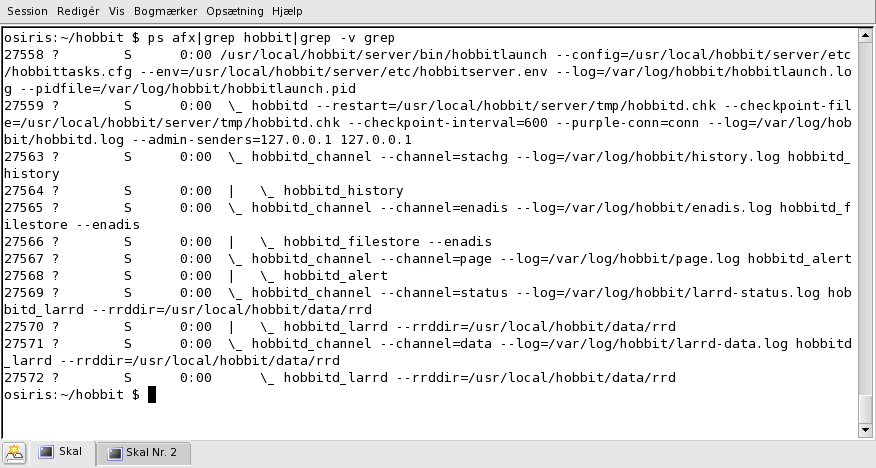
\includegraphics[scale=0.6]{./hobbitprocs.png} 
\end{figure}

 Quite a few, but all of them controlled by the master hobbitlaunch
 process. A quick run-down of what each of them does:

\begin{itemize}
\item hobbitd is the network daemon that receives status updates from
  the clients and the network test tool. It also provides the current
  status of all your systems to the tool that generates the webpages.

\item hobbitd\_channel provides the communication between hobbitd and
  all of the helper modules that implement other server-based
  functions.

\item hobbitd\_history takes care of recording the history of status
  changes for each item you monitor. This is used to track what has
  happened with a single status over time - when it was red, when it
  was green, what the error reported at 2:51 AM last Friday looked
  like. The history file format is compatible with the format used by
  the Big Brother package.

\item hobbitd\_filestore stores files with information about the
  current status of the systems monitored by Hobbit. There may be
  several of these running, but normally you will only need the one
  that stores information about hosts that have been disabled, which
  is the one you see here.

\item hobbitd\_alert takes care of sending out alerts when your
  servers begin to report a critical status.

\item hobbitd\_rrd updates the RRD database files with the numeric
  data collected from the status reports, to track e.g. how the disk
  utilization of a server changes over time. There are two of these
  processes, because the data can arrive in two different ways.


\end{itemize}


 After a couple of minutes, you should have data available for the
 Hobbit server itself. If you open a webbrowser with the Hobbit URL -
 usually \url{http://your.server/hobbit/} - you should see something
 like this:

\begin{figure} 
\centering \caption{hobbitmain.png}
\label{hobbitmain.png}
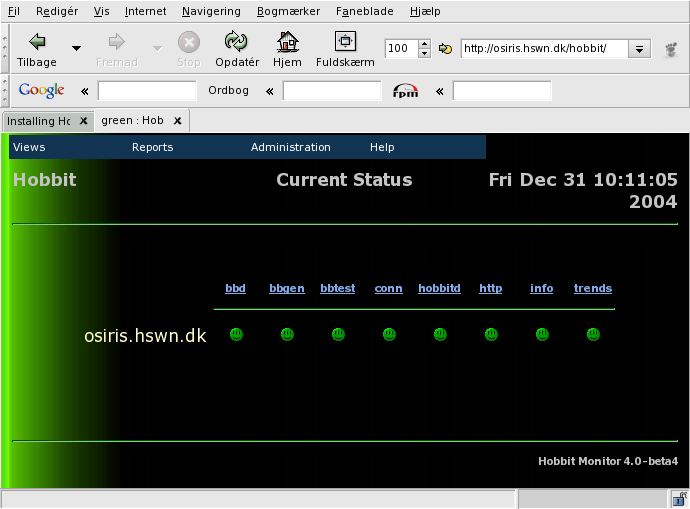
\includegraphics[scale=0.6]{./hobbitmain.png} 
\end{figure}


 Each of the little faces indicate an item that is being monitored for
 this host. Here you see the default set of items that the Hobbit
 installation sets up for a Hobbit server:

\begin{itemize}
\item \emph{bbd}
 is the availability of the Hobbit network daemon.
\item \emph{bbgen}
 is the status of the bbgen tool, which updates the webpages.
\item \emph{bbtest}
 is the status of the bbtest-net network tester that performs all of
 the network tests you configure in Hobbit.

\item \emph{conn}
 is a simple ``ping'' test of the host.
\item \emph{hobbitd}
 is the status of the Hobbit daemon, with statistics about how many
 monitored items are being tracked.

\item \emph{http}
 is the status of the HTTP-server running on the Hobbit server.
\item \emph{info}
 contains information about how the host is configured in Hobbit, such
 as what IP-address it has, what network tests are being run against
 this host etc.

\item \emph{trends}
 is a collection of the various RRD graphs available for this host.

\end{itemize}


 You can click on each of the green icons to see a more detailed status.
\subsection{Next steps}


 Congratulations, you now have a running Hobbit server!


 The next step is to configure it to monitor your servers and
 applications, and to set up the alerts to send you e-mail, call a
 pager, or send an SMS in case of trouble. For that, see the Hobbit
 configuration guide.





